\scanpage{14}

% Wholly handwritten page: the main hand is unnamed.
% The following clipped left-edge traces have no secure lexical identification.
% Their textual status is uncertain; the phantom alternatives do not deny the ink.
\reversemarginpar
\margin{\figure{\unsure{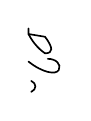
\begin{tikzpicture}[x=.35mm,y=.35mm,line width=.6pt,line cap=round]
\draw (0,16) -- (0,14) -- (6,13) .. controls (9,9) and (9,7) .. (6,7)
 .. controls (3,9) and (1,12) .. (0,14);
\draw (0,4) .. controls (5,0) and (10,-1) .. (11,1)
 .. controls (12,3) and (10,5) .. (7,5);
\draw (1,-3) .. controls (3,-4) and (3,-6) .. (1,-7);
\end{tikzpicture}|\phantom{\rule{4mm}{9mm}}}}}
\normalmarginpar
b) $\forall\,F$ injectif sur $\unsure{Y}$, $\unsure{g|q}^{*}(F)$ est injectif et $F\unsure{\mathord{-}|\to}g_{*}g^{*}F$ est un épimorphisme (ex: $g$ inclusion d'un ouvert $U\hookrightarrow e_{Y}$).
On prend
\[
\mathbb R\Gamma_{Y}\bigl(\operatorname{Ker}\bigl(\underbrace{C(F}_{\text{rés. inj.}})\to
g_{*}g^{*}\unsure{(|C}C(F)\bigr)\bigr)\bigr)
\]
% Small detached right-margin trace beside/below the first display; status uncertain.
\margin{\figure{\unsure{\begin{tikzpicture}[x=.35mm,y=.35mm,line width=.35pt,line cap=round]
\draw[gray] (0,5) .. controls (1,4) and (2,5) .. (3,5);
\fill (2,2.5) circle (.35);
\draw[gray] (2,2.2) -- (1.5,.5);
\fill[gray] (1,-1) ellipse (.3 and .65);
\end{tikzpicture}|\phantom{\rule{2mm}{4mm}}}}}

Dans le cas général, la difficulté provient du fait que le cône d'un morphisme de complexes (tel que
% Clipped left-edge upright, lower bar and point; no secure textual identity.
\reversemarginpar
\margin{\figure{\unsure{\begin{tikzpicture}[x=.35mm,y=.35mm,line width=.6pt,line cap=round]
\draw (0,8) -- (0,2);
\draw (0,0) -- (5,.4);
\fill (0,-5) ellipse (.45 and .7);
\end{tikzpicture}|\phantom{\rule{3mm}{6mm}}}}}
\normalmarginpar
\[
F\to g_{*}\deleted{\unsure{C|(}}\bigl(g^{*}(F)\deleted{\unsure{)|C}}\bigr)
\deleted{\unsure{*|g_{*}}}\qquad\text{)}
\]
n'est pas fonctoriel (dans la
% Detached dark left-edge point, textual status uncertain.
\reversemarginpar
\margin{$\unsure{\cdot|\phantom{\cdot}}$}
\normalmarginpar
catégorie dérivée) p. r. à la flèche dont on veut prendre le cône.

% Clipped curved trace at the left edge beside this paragraph.
\reversemarginpar
\margin{\figure{\unsure{\begin{tikzpicture}[x=.4mm,y=.4mm,line width=.6pt,line cap=round]
\draw (0,3) .. controls (4,1) and (4,-2) .. (0,-3);
\end{tikzpicture}|\phantom{\rule{2mm}{3mm}}}}}
\normalmarginpar
Et pourtant, dans le cas particulier actuel\unsure{\phantom{,}|,} il devrait y avoir un choix fonctoriel.
% The detached point lies below-left of the hyphen between t and ce.
\unsure{ESt|Est}$\underset{\hspace{-.35em}\unsure{\cdot|\phantom{\cdot}}}{\text{-}}$ce
\unsure{\.{e}vident|évident|evident} ?
\textsuperscript{\unsure{'|\phantom{'}}}
% A further clipped curved trace lies at the left edge beside the preceding question.
\reversemarginpar
\margin{\figure{\unsure{\begin{tikzpicture}[x=.4mm,y=.4mm,line width=.6pt,line cap=round]
\draw (0,3) .. controls (3,1) and (3,-2) .. (0,-3);
\end{tikzpicture}|\phantom{\rule{2mm}{3mm}}}}}
\normalmarginpar

\unsure{Q\uline{uestion pour Illusi}e|Q\uline{uestion pour Illusie}} : Dans sa théorie des déform.tions de schémas en \unsure{groupes|groupe}
% Clipped left-edge thick curved trace and small lower point.
\reversemarginpar
\margin{\figure{\unsure{\begin{tikzpicture}[x=.4mm,y=.4mm,line width=.8pt,line cap=round]
\draw (0,3) .. controls (2,1) and (2,0) .. (0,-1);
\fill (0,-6) ellipse (.25 and .4);
\end{tikzpicture}|\phantom{\rule{2mm}{4mm}}}}}
\normalmarginpar
plats, il tombe sur des $H^{3}(B_{\unsure{G|C}}/X,\quad)$ resp. des $\operatorname{Ext}^{2}(\unsure{K|X};,\quad)$.
Peut-on courtcircuiter sa théorie via la théorie (supposée écrite) des Gr-champs - resp. via la théorie des champs de Picard ? J'ai

% Two detached bottom points, below the faint horizontal paper/image rule.
\begin{center}
$\unsure{\bullet\,\cdot|\phantom{\bullet\,\cdot}}$
\end{center}
% The faint horizontal gray rule near the foot is not assigned a textual function.
% archive sheet number: 13

